\documentclass{standalone}
%\usepackage{import}
%\subimport{.../}{preamble}
\usepackage{tikz, graphicx, cmbright}
\begin{document}
\fontsize{10pt}{1em}\selectfont

\begin{tikzpicture}
\node [above right] at (0, 0) {\includegraphics{simple_optics_dimer_layout.png}};
{\fontsize{9pt}{1em}\selectfont
{\color{white} \node [align=center] at (3.5, 7.9) {$100\times$\,IR\\obj.};}}
\node [align=center] at (1.3, 9.4) {coarse $xyz$\\nanopositioning};
\node [align=center] at (5.7, 9.4) {fine (piezo) $xyz$\\nanopositioning};
\node [align=center] at (4, 9.5) {$dz$};
\node [align=center] at (1.35, 8.4) {$V$};
\node [align=center] at (5.6, 8.4) {$I$};
\node [align=center] at (8.5, 9) {AFM: cantilever\\deflection};
\node at (2.3, 6.2) {reimaging};
\node [align=left] at (1.5, 5.4) {supercontinuum\\illumination};
\node at (1.4, 3.0) {to CCD};
\node [align=center] at (5.4, 1.8) {confocal\\pinhole};
\node [align=center] at (7.4, 2.5) {transverse\\polarisation};
\node [align=center] at (8.9, 1.4) {axial\\polarisation};
\end{tikzpicture}

\end{document}